% Created 2022-09-19 Mon 08:37
% Intended LaTeX compiler: pdflatex
\documentclass[presentation,aspectratio=169, usenames, dvipsnames]{beamer}
\usepackage[utf8]{inputenc}
\usepackage[T1]{fontenc}
\usepackage{graphicx}
\usepackage{grffile}
\usepackage{longtable}
\usepackage{wrapfig}
\usepackage{rotating}
\usepackage[normalem]{ulem}
\usepackage{amsmath}
\usepackage{textcomp}
\usepackage{amssymb}
\usepackage{capt-of}
\usepackage{hyperref}
\usepackage{khpreamble}
\usepackage{amssymb}
\usepgfplotslibrary{groupplots}
\newcommand*{\shift}{\operatorname{q}}
\definecolor{ppc}{rgb}{0.1,0.1,0.6}
\definecolor{iic}{rgb}{0.6,0.1,0.1}
\definecolor{ddc}{rgb}{0.1,0.6,0.1}
\usetheme{default}
\author{Kjartan Halvorsen}
\date{\today}
\title{Design of control systems}
\hypersetup{
 pdfauthor={Kjartan Halvorsen},
 pdftitle={Design of control systems},
 pdfkeywords={},
 pdfsubject={},
 pdfcreator={Emacs 26.3 (Org mode 9.4.6)}, 
 pdflang={English}}
\begin{document}

\maketitle

\section{Course content}
\label{sec:org971d020}

\begin{frame}[label={sec:org680b461}]{Feedback control systems are ubiquitous}
\begin{center}
  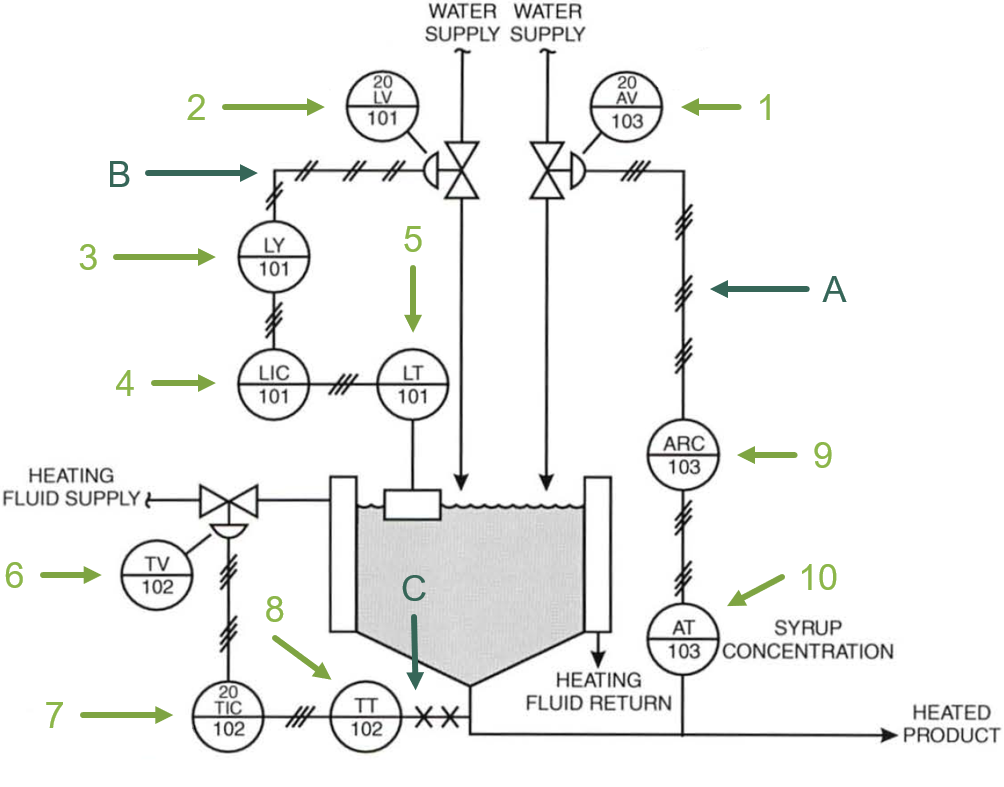
\includegraphics[width=.6\linewidth]{../../figures/PnID-ex.png}
\end{center}
\end{frame}

\begin{frame}[label={sec:orgc3a170a}]{Feedback control systems}
The problem situation

\begin{center}
  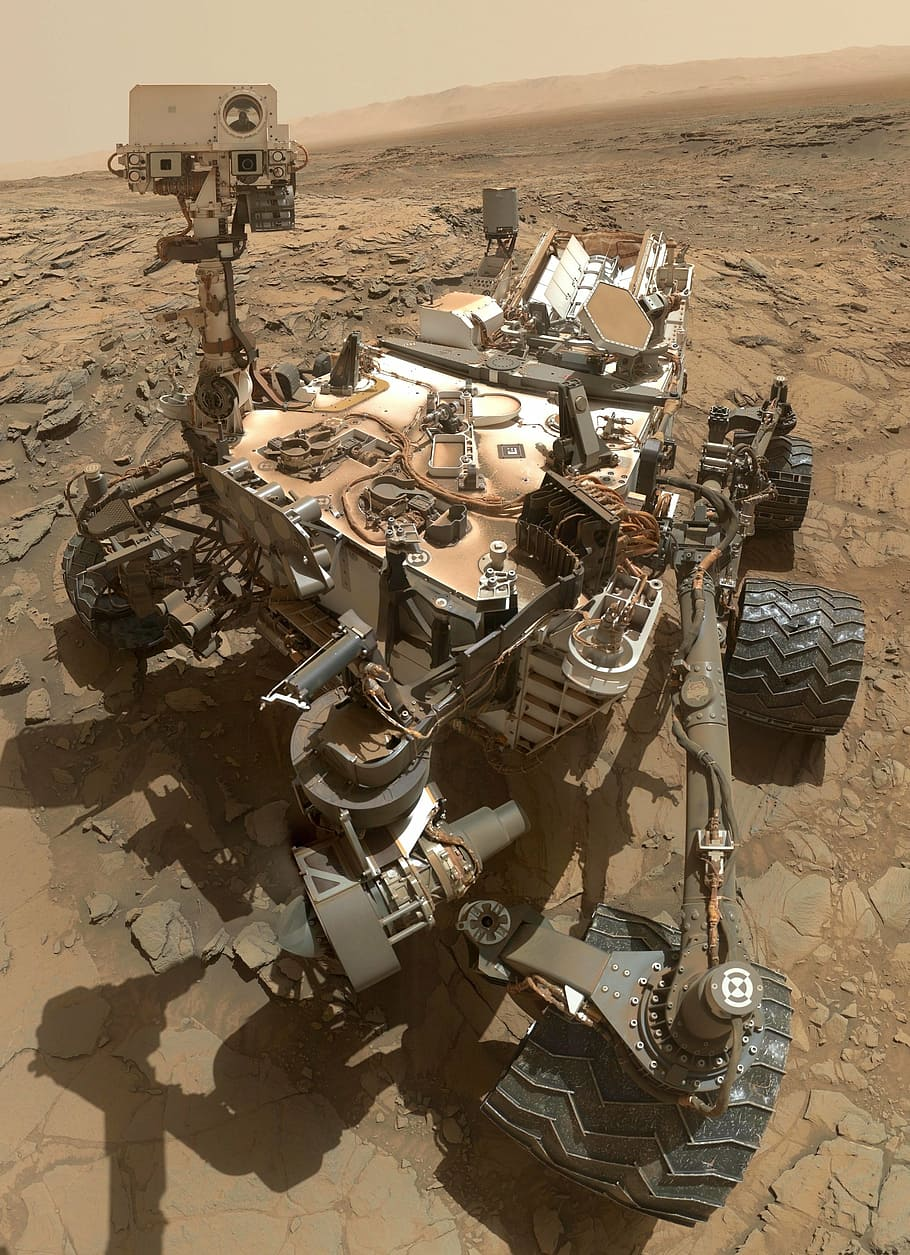
\includegraphics[width=.34\linewidth]{../../figures/mars-rover-curiosity-vehicle-cosmos.jpg}
\end{center}
\end{frame}


\begin{frame}[label={sec:orgcf586fe}]{Feedback control system}
\begin{columns}
\begin{column}{0.4\columnwidth}
\begin{center}
 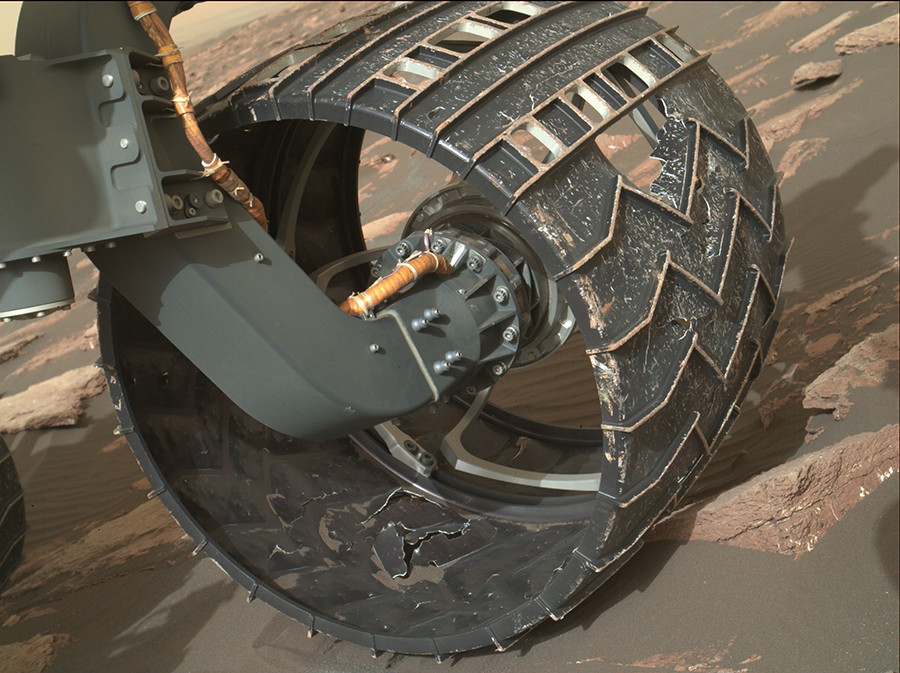
\includegraphics[width=1.0\linewidth]{../../figures/curiosity-wheel.jpg}
\end{center}
\end{column}

\begin{column}{0.6\columnwidth}
\pause

\begin{center}
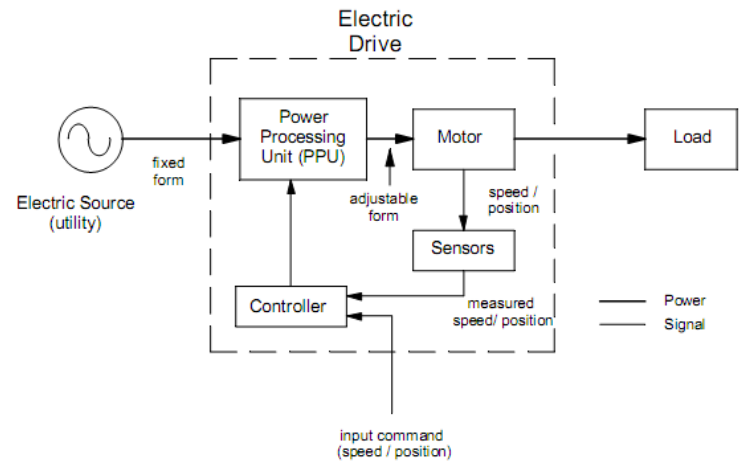
\includegraphics[width=\linewidth]{../../figures/electric-drive-block.png}
\end{center}
\end{column}
\end{columns}
\end{frame}




\section{Control systems specifications}
\label{sec:org1715818}

\begin{frame}[label={sec:orgab5ae99}]{Performance requirements - time domain}
\begin{center}
  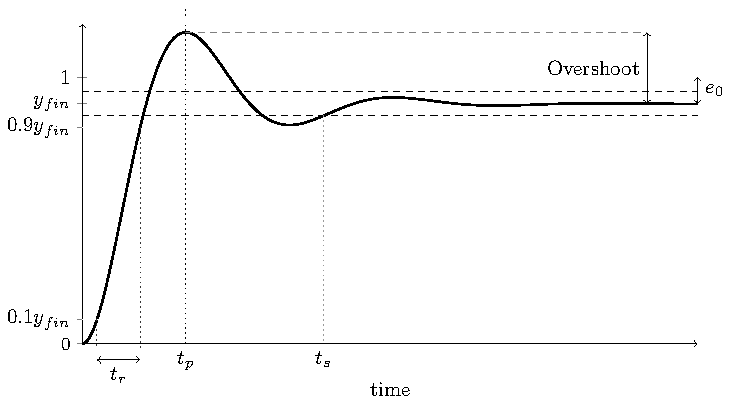
\includegraphics[width=.8\linewidth]{../../figures/step-response-specifications}
\end{center}
\end{frame}

\begin{frame}[label={sec:org704aa58}]{Performance requirements - time domain}
\alert{Activity} Does the system satisfy the requirements?

\begin{columns}
\begin{column}{0.3\columnwidth}
\begin{center}
\begin{tabular}{ll}
Rise time & < 1.5s\\
Overshoot & < 18\%\\
\end{tabular}
\end{center}
\end{column}


\begin{column}{0.7\columnwidth}
\begin{center}
 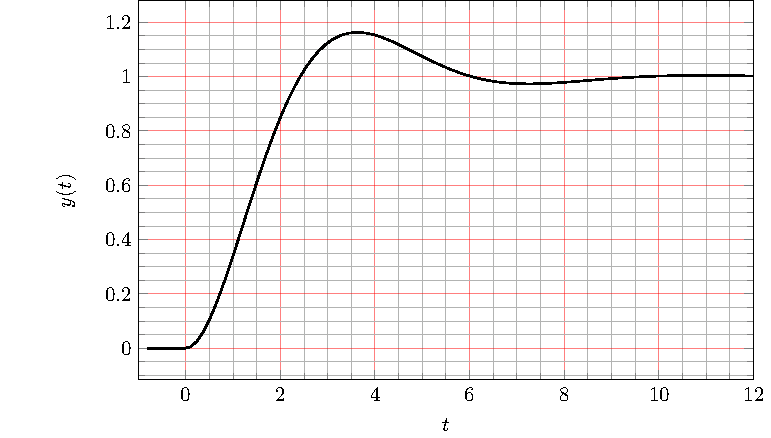
\includegraphics[width=1.0\linewidth]{../../figures/second-order-response-example}
\end{center}
\end{column}
\end{columns}
\end{frame}
\begin{frame}[label={sec:orge5710ca}]{Performance requirements - frequency domain}
\begin{center}
  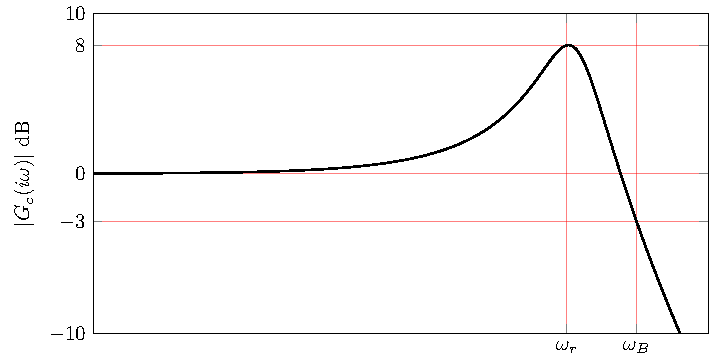
\includegraphics[width=.8\linewidth]{../../figures/spec-bode-closed-loop-new}
\end{center}
\end{frame}


\begin{frame}[label={sec:orgfd2f2c4}]{Performance requirements - frequency domain}
\begin{center}
  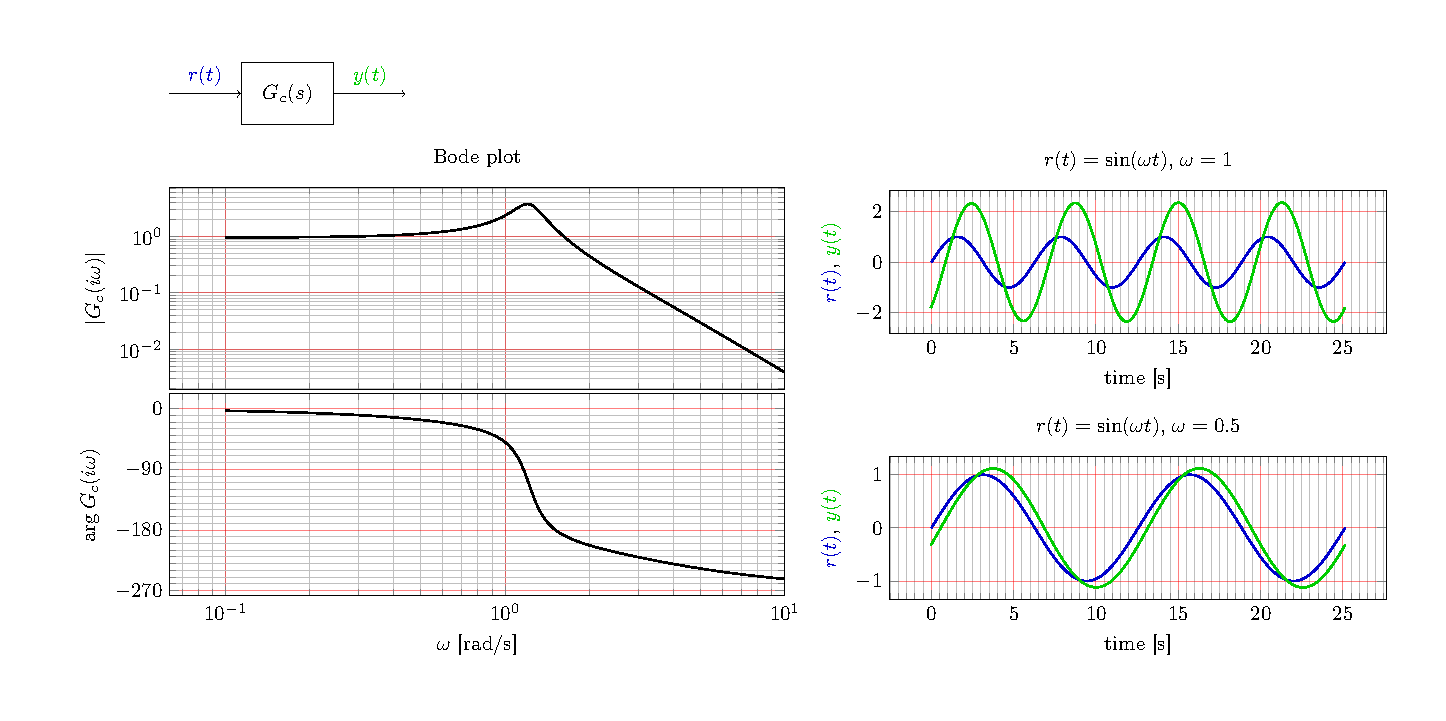
\includegraphics[width=1.0\linewidth]{../../figures/bode-closed-loop-example-responses}
\end{center}

\pause

\alert{Activity} What is the gain and phase shift at \(\omega = 2\) rad/s?
\end{frame}

\begin{frame}[label={sec:org8f6776f}]{Performance requirements - frequency domain}
\begin{center}
  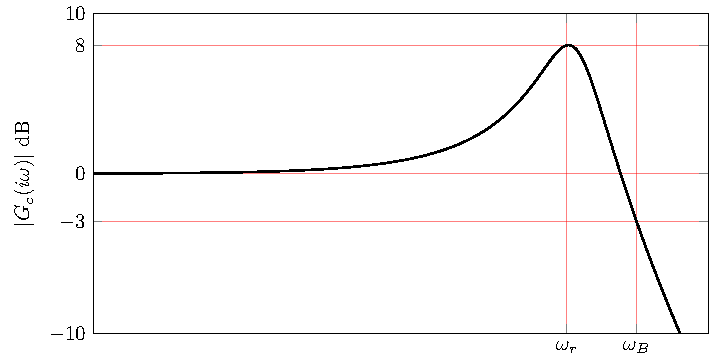
\includegraphics[width=.8\linewidth]{../../figures/spec-bode-closed-loop-new}
\end{center}
\end{frame}


\begin{frame}[label={sec:org37174b6}]{Performance requirements - frequency domain}
\alert{Activity} Does the system satisfy the requirements?


\begin{columns}
\begin{column}{0.7\columnwidth}
\begin{center}
 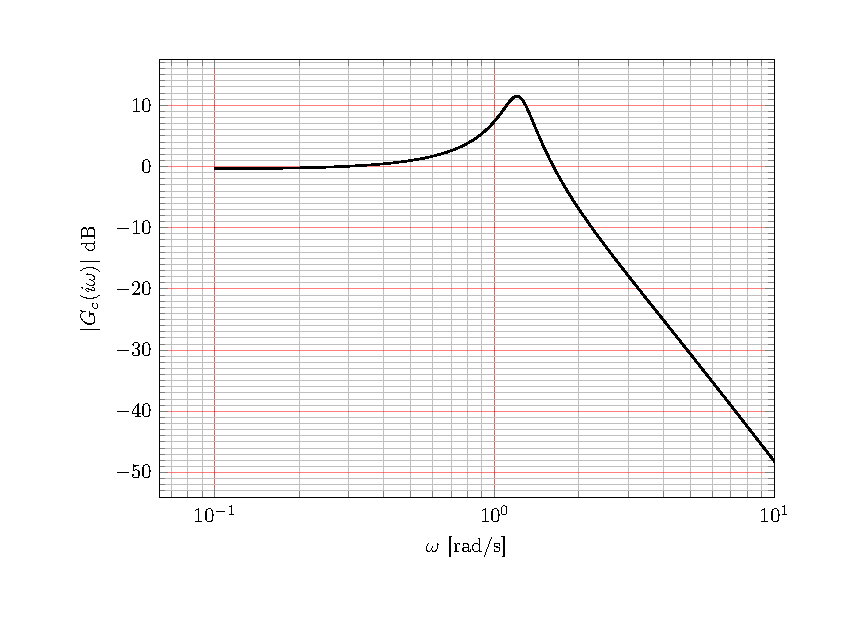
\includegraphics[width=1.0\linewidth]{../../figures/bode-closed-loop-example}
\end{center}
\end{column}
\begin{column}{0.3\columnwidth}
\begin{center}
\begin{tabular}{ll}
Bandwidth & >3 rad/s\\
Resonance peak & <9dB\\
\end{tabular}
\end{center}
\end{column}
\end{columns}
\end{frame}




\section{Feedback, sensitivity and complementary sensitivity}
\label{sec:org4454ec2}

\begin{frame}[label={sec:orga1227ac}]{Block diagram algebra}
\begin{center}
  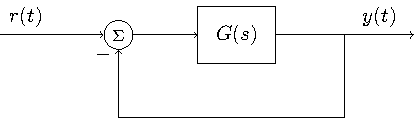
\includegraphics[width=.6\linewidth]{../../figures/block-simple-feedback}
\end{center}

Transfer function from \(r(t)\) to \(y(t)\):
\[ \frac{Y(s)}{R(s)} = \frac{G(s)}{ 1+ G(s)}\]
\end{frame}


\begin{frame}[label={sec:org81dbfff}]{Block diagram algebra}
\alert{Activity} Pair the block-diagram with the correct closed-loop transfer function!


\begin{longtable}{cccc}
\textcolor{red}{A} & \textcolor{red}{B} & \textcolor{red}{C} & \textcolor{red}{D}\\
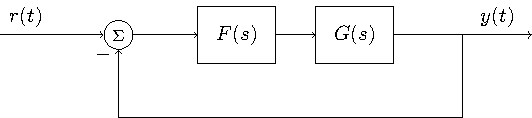
\includegraphics[width=3cm]{../../figures/block-simple-control-feedback} & 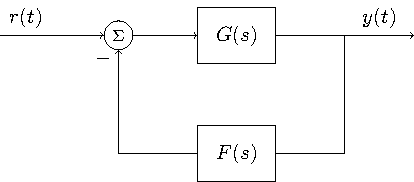
\includegraphics[width=3cm]{../../figures/block-simple-control-feedback2} & 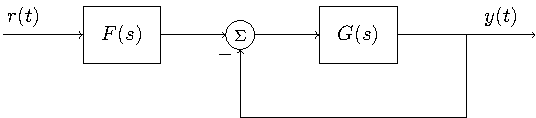
\includegraphics[width=3cm]{../../figures/block-simple-control-feedback3} & 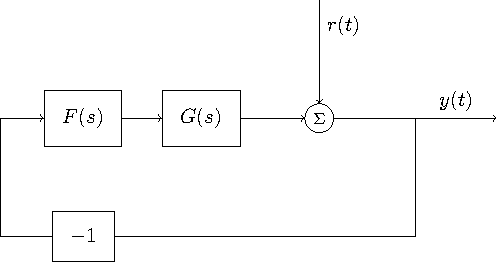
\includegraphics[width=3cm]{../../figures/block-simple-control-feedback4}\\
\end{longtable}


\begin{longtable}{cccc}
\textcolor{blue!80!black}{I} & \textcolor{blue!80!black}{II} & \textcolor{blue!80!black}{III} & \textcolor{blue!80!black}{IV}\\
\(\frac{Y(s)}{R(s)}=\frac{G(s)F(s)}{1 + G(s)}\) & \(\quad \frac{Y(s)}{R(s)}=\frac{G(s)}{1 + G(s)F(s)}\quad\) & \(\frac{Y(s)}{R(s)}=\frac{1}{1 + G(s)F(s)}\) & \(\frac{Y(s)}{R(s)}=\frac{G(s)F(s)}{1 + G(s)F(s)}\)\\
\end{longtable}
\end{frame}
\end{document}